Now having two models for the predictions of two organelles: nuclei and ER it is interesting to visualize the predictions together (see Figure \ref{fig:er-combined}). It is clear from the image that ER indeed is located around the nucleus. Unfortunately the cells were stained only for separate oragnelles and different fluorescent target do not intersect, meaning there were no images with both nucleus and ER stained together. This would be a field where further research can be applied as having such data would allow to evaluate the models event better measuring the intersection error between the two for instance.
\begin{figure}[htb]
    \centering
    \setkeys{Gin}{width=\linewidth}
    \centering
        \begin{tabularx}{\textwidth}{YYYY}
            \textbf{Ground truth} &
            \textbf{Prediction} &
            \textbf{Prediction + nuclei} \\
            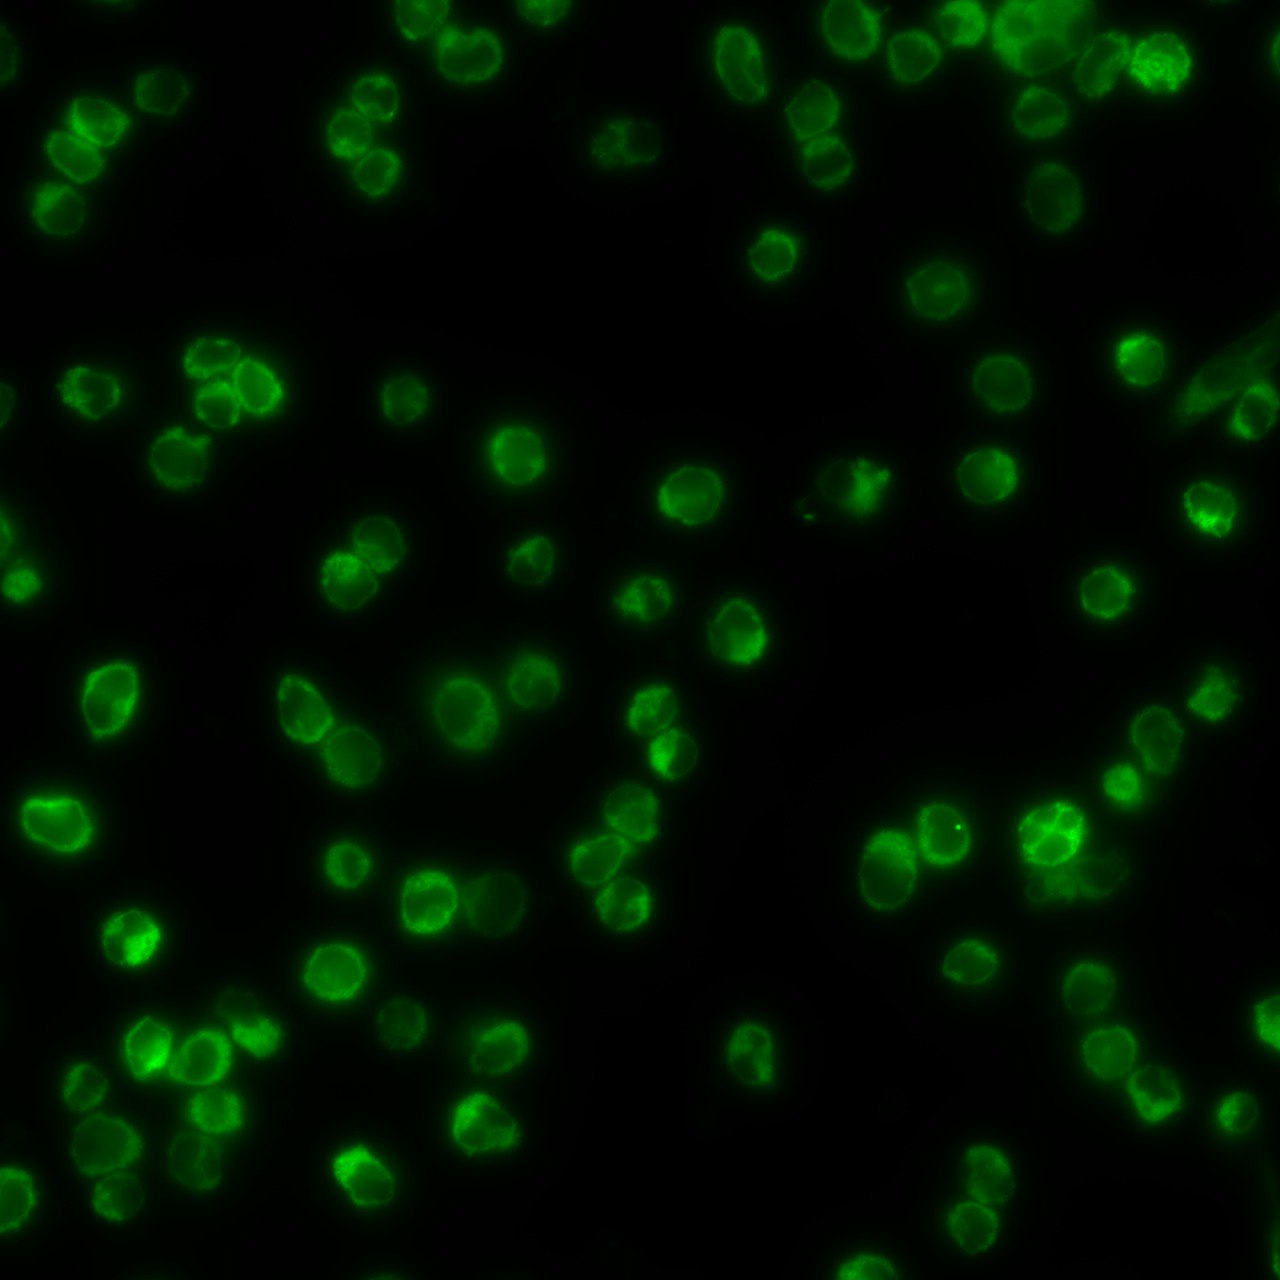
\includegraphics{bilder/ER/gt.jpg} & 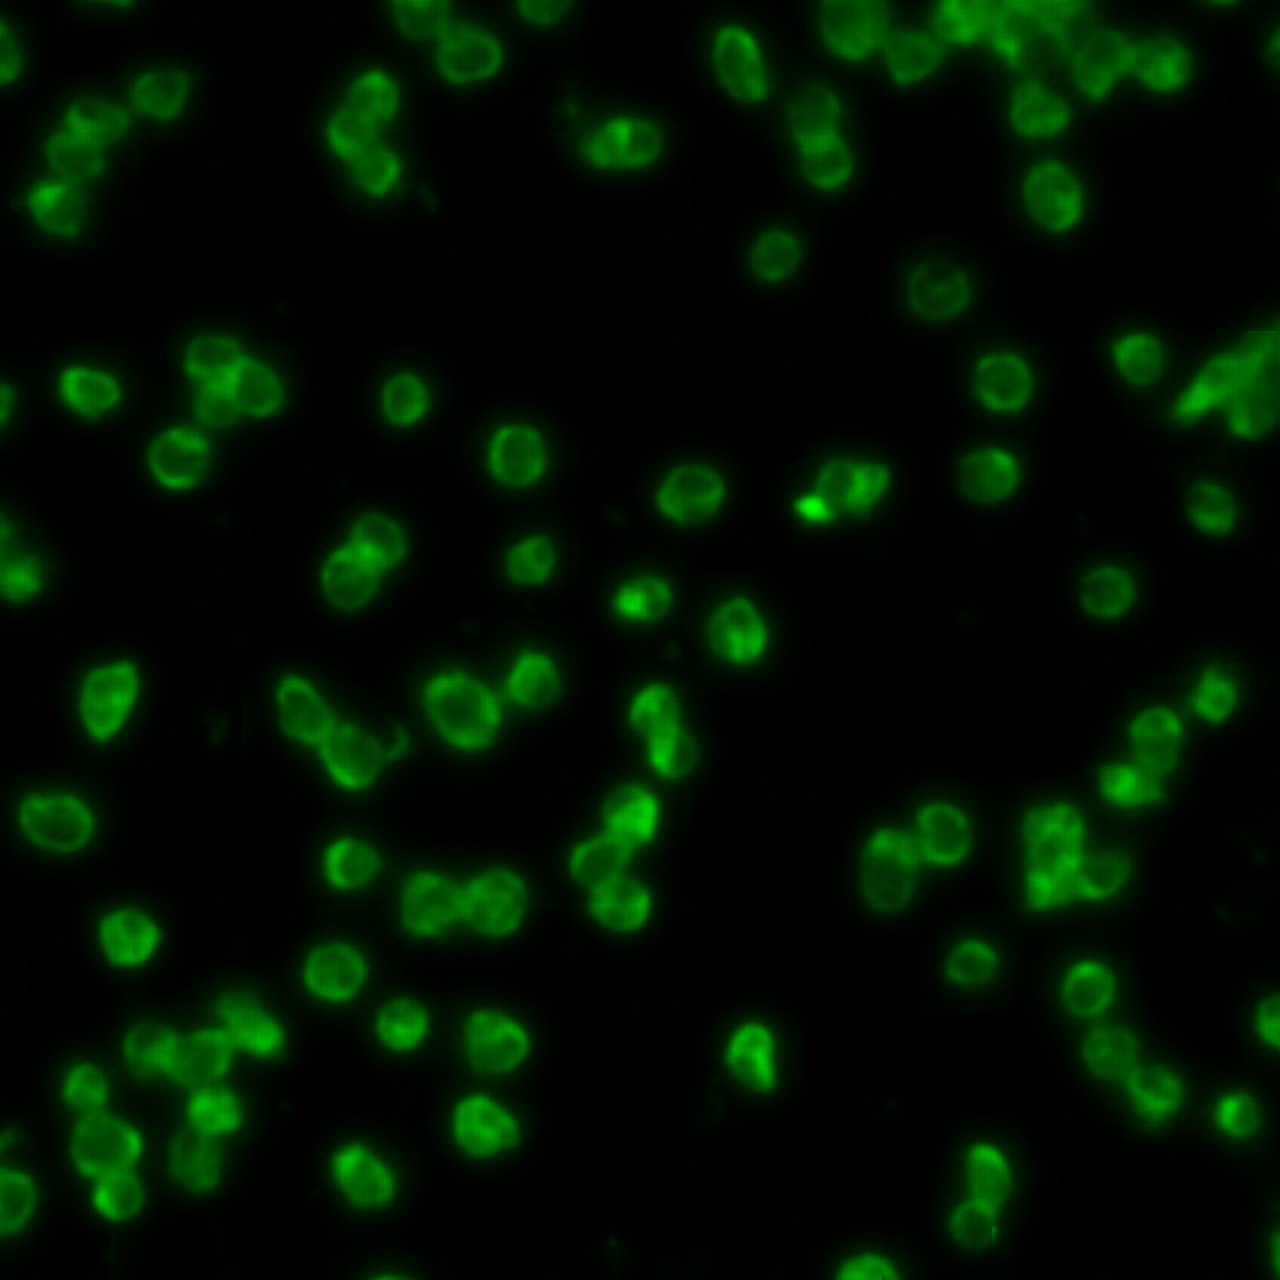
\includegraphics{bilder/ER/er.jpg} &
            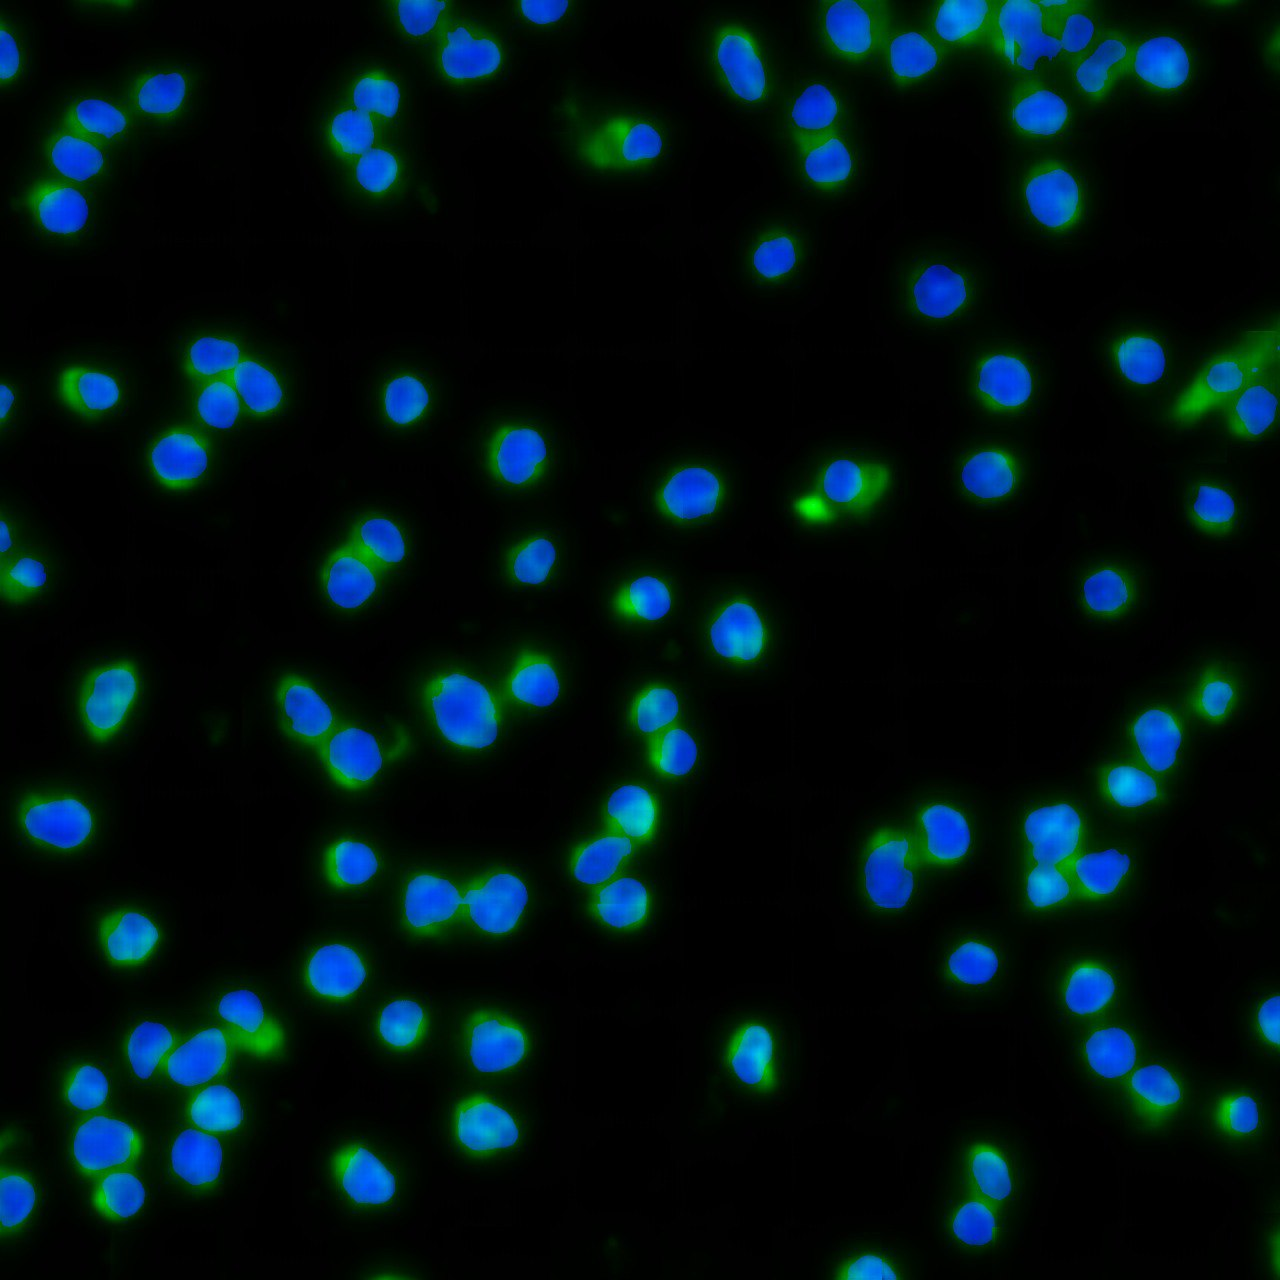
\includegraphics{bilder/ER/gt_nuclei.jpg}
        \end{tabularx}
    \caption{Combination pof ER with nuclei}
    \label{fig:er-combined}
\end{figure}